\chapter{Foundations of Multi-Agent Reinforcement Learning}

\section*{Introduction}
Multi-agent reinforcement learning (MARL) is, in essence, reinforcement learning (RL) applied to multi-agent game models to learn optimal policies for the agents. Thus, MARL is deeply rooted in both RL theory and game theory. This chapter provides the necessary theoretical background, starting with the foundational principles of single-agent RL before extending them to the multi-agent domain.

\section{Single-Agent Reinforcement Learning}
To understand how multiple agents learn and interact, we must first understand how a single agent learns. This section introduces the theory and algorithms of RL when there is only a single agent for which we want to learn an optimal policy. We will begin by providing a general definition of RL, following which we will introduce the Markov decision process (MDP) as the foundational model used in RL to represent single-agent decision processes. Based on the MDP model, we will define basic concepts such as expected returns, optimal policies, value functions, and Bellman equations. Most of the MARL algorithms introduced later in this chapter build on these concepts and essentially extend them to multi-agent game models.
\begin{figure}[!ht]
    \centering
    % This is a placeholder for your figure. 
     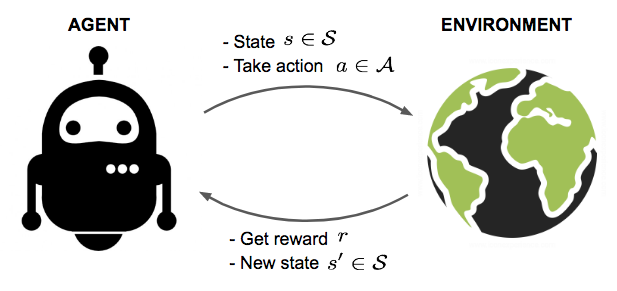
\includegraphics[width=0.48\textwidth]{img_pfe/RL_illustration.png}
    % \fbox{\rule{0pt}{4in} \rule{0.9\linewidth}{0pt}} 
    \caption{An agent interacts with the environment, trying to take smart actions to maximize cumulative rewards.}
    \label{fig:rl}
\end{figure}

\subsection*{General Definition of Reinforcement Learning}
We begin by providing a general definition of reinforcement learning:
\begin{quote}
    \textit{Reinforcement learning algorithms learn solutions for sequential decision processes via repeated interaction with an environment.} 
\end{quote}
This definition raises three main questions:
\begin{enumerate}
    \item What is a sequential decision process?
    \item What is a solution to the process?
    \item What is learning via repeated interaction?
\end{enumerate}

A sequential decision process is defined by an agent that makes decisions over multiple time steps within an environment to achieve a specified goal. In each time step, the agent receives an observation from the environment and chooses an action. Given the chosen action, the environment may change its state according to some transition dynamics and send a scalar reward signal to the agent. This fundamental interaction is often visualized as the RL loop.
\begin{figure}[h!]
\centering

 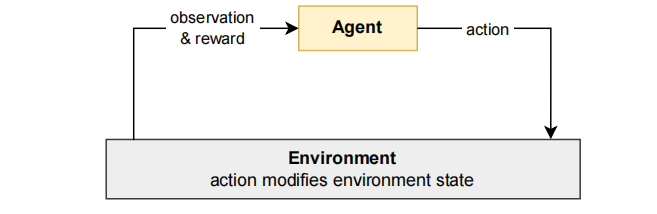
\includegraphics[width=0.8\textwidth]{img_pfe/rl_loop.PNG}
\caption{Basic reinforcement learning loop for a single-agent system.}
\label{fig:rl_loop}
\end{figure}



A solution to the decision process is an optimal decision policy for the agent, which chooses actions in each state to achieve some specified learning objective. Typically, the learning objective is to maximize the expected return for the agent in each possible state. The return is defined as the sum of rewards received over time.

Finally, RL algorithms learn via repeated interaction by trying different actions in different states and observing the outcomes. This method is often described as “trial and error.” A central problem in this learning process is the exploration-exploitation dilemma: how to balance exploring the outcomes of different actions versus sticking with (exploiting) actions that are currently believed to be best.

RL is a distinct type of machine learning. It is not supervised learning, because reward signals do not directly tell the agent which action to take. It also differs from unsupervised learning because the rewards, while not a supervised signal, act as feedback from which to learn an optimal policy. In the following sections, we will formally define these concepts within the framework of the Markov decision process.

\subsection*{Markov Decision Processes (MDPs)}
The standard model used in RL to formalize the sequential decision process is the Markov decision process.

\begin{definition}[Markov decision process]
A finite MDP consists of:
\begin{itemize}
    \item A finite set of states $\mathcal{S}$
    \item A finite set of actions $\mathcal{A}$
    \item A reward function $R: \mathcal{S} \times \mathcal{A} \times\mathcal{S} \rightarrow \mathbb{R}$
    \item A state transition probability function $T: \mathcal{S} \times \mathcal{A} \times \mathcal{S} \rightarrow [0,1]$
    \item An initial state distribution $\mu: \mathcal{S} \rightarrow [0,1]$
\end{itemize}
\end{definition}

At each time step $t$, the agent observes the current state $s_t \in \mathcal{S}$ and chooses an action $a_t \in \mathcal{A}$ according to its policy, $\pi(a_t | s_t)$. The MDP then transitions to a next state $s_{t+1}$ with probability $T(s_{t+1} | s_t, a_t)$, and the agent receives a reward $r_t = R(s_t, a_t, s_{t+1})$. This process continues until a terminal state is reached.

The term “Markov” comes from the Markov property, which states that the future is conditionally independent of the past, given the present state and action:
$$
\Pr(s_{t+1}, r_t | s_t, a_t, s_{t-1}, a_{t-1}, \dots, s_0, a_0) = \Pr(s_{t+1}, r_t | s_t, a_t)
$$

This means the current state provides all necessary information to make an optimal decision. The most common assumption in RL is that the dynamics of the MDP (the transition and reward functions) are a priori unknown to the agent.

An important special case of the MDP is the Partially Observable Markov Decision Process (POMDP), where the agent receives an observation $o_t$ rather than the true state $s_t$. POMDPs are a special case of the multi-agent models we will introduce later.

\subsection*{Expected Discounted Returns and Optimal Policies}
We have defined the MDP as a model of the decision process, but we must also define the learning objective. The most common objective is maximizing the expected discounted return.

Given that an episode may run for a long time or even indefinitely, future rewards are typically discounted by a factor $\gamma \in [0, 1)$. The discounted return is defined as:
\begin{equation}
G_t = \sum_{k=0}^{\infty} \gamma^k r_{t+k}
\end{equation}

The discount factor ensures that the sum of rewards is finite.

\subsection*{Value Functions and the Bellman Equation}
The Markov property of the decision process allows us to define the expected return on a state-by-state basis. This gives rise to the concept of value functions, which are fundamental to Reinforcement Learning. They estimate how good it is to be in a particular state, or to take a particular action in a state.

First, we can express the discounted return, $G_t$, in a recursive form:
\begin{equation}
    G_t = r_t + \gamma r_{t+1} + \gamma^2 r_{t+2} + \cdots = r_t + \gamma G_{t+1}
\end{equation}

Given a policy $\pi$, which specifies the probability $\pi(a|s)$ of taking action $a$ in state $s$, we can define two types of value functions:

\paragraph{The State-Value Function ($V^\pi$):}
This function gives the expected return when starting in state $s$ and following policy $\pi$ thereafter. It is defined as:
\begin{equation}
    V^\pi(s) = \mathbb{E}_\pi[G_t | S_t = s]
\end{equation}

The state-value function adheres to a recursive relationship known as the Bellman equation:
\begin{equation}
    V^\pi(s) = \sum_{a \in \mathcal{A}} \pi(a|s) \sum_{s' \in \mathcal{S}} P(s'|s,a)[R(s,a,s') + \gamma V^\pi(s')]
\end{equation}

For a finite state space, this equation forms a system of linear equations whose unique solution is the value function $V^\pi$.

\paragraph{The Action-Value Function ($Q^\pi$):}
This function gives the expected return after taking a specific action $a$ in state $s$ and then following policy $\pi$. It is defined as:
\begin{equation}
    Q^\pi(s,a) = \mathbb{E}_\pi[G_t | S_t = s, A_t = a]
\end{equation}

Similar to the state-value function, $Q^\pi$ satisfies its own Bellman equation:
\begin{equation}
    Q^\pi(s,a) = \sum_{s' \in \mathcal{S}} P(s'|s,a)[R(s,a,s') + \gamma V^\pi(s')]
\end{equation}

By substituting $V^\pi(s') = \sum_{a' \in \mathcal{A}} \pi(a'|s') Q^\pi(s',a')$, we can express the Bellman equation for $Q^\pi$ solely in terms of action-values:
\begin{equation}
    Q^\pi(s,a) = \sum_{s' \in \mathcal{S}} P(s'|s,a) \left[ R(s,a,s') + \gamma \sum_{a' \in \mathcal{A}} \pi(a'|s') Q^\pi(s',a') \right]
\end{equation}

\subsection*{Optimal Value Functions and Policies}
The ultimate goal in an MDP is to find an optimal policy, denoted $\pi^*$, that maximizes the expected return. A policy is considered optimal if its expected return is greater than or equal to that of all other policies for all states. Such a policy shares a unique optimal value function.

The optimal state-value function, $V^*(s)$, and optimal action-value function, $Q^*(s,a)$, are defined as:
\begin{align}
    V^*(s) &= \max_{\pi} V^\pi(s), \quad \forall s \in \mathcal{S} \\
    Q^*(s,a) &= \max_{\pi} Q^\pi(s,a), \quad \forall s \in \mathcal{S}, a \in \mathcal{A}
\end{align}

These optimal value functions satisfy a special set of recursive equations called the Bellman optimality equations. Unlike the standard Bellman equations, these are non-linear due to the maximization operator.

The Bellman optimality equation for $V^*$ is:
\begin{equation}
    V^*(s) = \max_{a \in \mathcal{A}} \sum_{s' \in \mathcal{S}} P(s'|s,a) [R(s,a,s') + \gamma V^*(s')]
\end{equation}

And for $Q^*$:
\begin{equation}
    Q^*(s,a) = \sum_{s' \in \mathcal{S}} P(s'|s,a) \left[ R(s,a,s') + \gamma \max_{a' \in \mathcal{A}} Q^*(s',a') \right]
\end{equation}

Solving this system of non-linear equations provides the optimal action-value function, $Q^*$. Once $Q^*$ is known, the optimal policy $\pi^*$ can be derived by deterministically selecting the action with the maximum value in each state:
\begin{equation}
    \pi^*(s) = \arg\max_{a \in \mathcal{A}} Q^*(s,a)
\end{equation}

While the optimal value function is unique for a given \textit{MDP}, there can be multiple optimal policies that achieve this same maximum value. The existence of a solution to the Bellman optimality equation guarantees that there is always at least one deterministic optimal policy. The methods for solving these equations, such as dynamic programming and temporal-difference learning, are central to finding solutions for reinforcement learning problems.
% \subsection{Methods for Solving MDPs}
% Now that we have formally defined the components of an MDP and the objective of finding an optimal policy, we turn our attention to the algorithms designed to solve for $V^*$ and $\pi^*$. These methods provide the computational foundation for reinforcement learning. We begin with methods that require a complete model of the environment.
%---- old dynamic --------
% \subsection*{Dynamic Programming}
% Dynamic Programming (DP) is a collection of algorithms that compute optimal policies given a perfect model of an MDP, meaning the transition probabilities $T(s'|s, a)$ and the reward function, $R(s, a,s')$, must be fully known.

% DP is foundational because it turns the Bellman equations into iterative update rules to find optimal value functions. Key DP methods like Policy Iteration and Value Iteration introduce the concept of bootstrapping—updating a state's value estimate based on the values of its successor states, which is a core property of many RL algorithms.

% \paragraph{Policy Iteration}
% Policy iteration finds the optimal policy $\pi^*$ by alternating between two steps: policy evaluation and policy improvement. It starts with an initial policy $\pi_0$ and refines it until it converges.

% The process follows this pattern:
% $$ \pi_0 \xrightarrow{\text{evaluate}} V^{\pi_0} \xrightarrow{\text{improve}} \pi_1 \xrightarrow{\text{evaluate}} V^{\pi_1} \xrightarrow{\text{improve}} \pi_2 \rightarrow \dots \rightarrow \pi^* $$

% \begin{enumerate}
%     \item \textbf{Policy Evaluation:} For the current policy $\pi$, we compute the state-value function $V^\pi$. This is done by iteratively applying the Bellman equation as an update rule, starting with an arbitrary value function $V_0$:
%     \begin{equation}
%     V_{k+1}(s) \leftarrow \sum_{a \in A} \pi(a|s) \sum_{s' \in S} T(s'|s,a) [R(s,a,s') + \gamma V_k(s')] 
%     \end{equation}
%     This process is guaranteed to converge to the true value function $V^\pi$. This is because the Bellman operator is a $\gamma$-contraction mapping, which, by the Banach fixed-point theorem, ensures convergence to a unique fixed point.

%     \item \textbf{Policy Improvement:} Once $V^\pi$ is computed, the policy is improved by making it greedy with respect to the value function. For each state, the new policy $\pi'$ greedily selects the best action:

%     \begin{equation}
%     \pi^{'}(s)  \leftarrow \arg\max_{a \in A} \sum_{s' \in S} T(s'|s,a) [R(s,a,s') + \gamma V^\pi(s')]
%    \end{equation}
%     Thanks to the policy improvement theorem, this new policy $\pi'$ is guaranteed to be as good as, or better than, $\pi$.
% \end{enumerate}

% These two steps are repeated until the policy is stable (i.e., $\pi' = \pi$), which indicates that the policy is optimal and satisfies the Bellman optimality equation.

% \paragraph{Value Iteration}
% This method merges policy evaluation and improvement into a single step. Starting with an initial value function $V_0(s)$, it repeatedly updates it using the Bellman optimality equation:
% $$ V_{k+1}(s) \leftarrow \max_{a \in A} \sum_{s' \in S} T(s'|s,a) [R(s,a,s') + \gamma V_k(s')] $$
% The process continues until the value changes are below a threshold. The optimal policy is then extracted by selecting the action that maximizes the expected return in each state:
% $$ \pi^*(s) \leftarrow \arg\max_{a \in A} \sum_{s' \in S} T(s'|s,a) [R(s,a,s') + \gamma V^*(s')] $$
% Value iteration is often faster than policy iteration since it avoids full evaluation of intermediate policies.
% \subsection*{Temporal-Difference Learning}
% While Dynamic Programming provides a solid foundation for solving MDPs, its requirement of a complete model of the environment ($T$ and $R$) is a significant limitation. In most real-world scenarios, the agent does not know the underlying dynamics. Temporal-Difference (TD) learning is a central concept in RL that allows an agent to learn directly from raw experience, making it a model-free approach.

% Like DP, TD learning uses bootstrapping to update value estimates based on other learned estimates. However, instead of sweeping through the entire state space, it learns from incomplete episodes, updating its knowledge after each time step. The agent interacts with the environment by executing an action $a_t$ from a state $s_t$, receiving a reward $r_t$, and observing the next state $s_{t+1}$. This experience tuple, $(s_t, a_t, r_t, s_{t+1})$, is used to update the action-value function, $Q(s_t, a_t)$.

% The general update rule for TD learning is:
% $$ Q(s_t, a_t) \leftarrow Q(s_t, a_t) + \alpha[\text{TD Target} - Q(s_t, a_t)] $$
% Here, $\ alpha\in [0,1]$ is the learning rate, and the TD Target is an estimate of the return that the agent aims to achieve. The term $\text{TD Target} - Q(s_t, a_t)$ is known as the TD error. The two most fundamental TD algorithms, Sarsa and Q-learning, differ in how they define this target.

% A critical challenge in model-free learning is the exploration-exploitation dilemma. To find the optimal policy, the agent must exploit actions it knows to be good, but it must also explore other actions to discover potentially better ones. A common solution is the $\epsilon$-greedy policy, where the agent chooses the best-known action with probability $1-\epsilon$ and a random action with probability $\epsilon$. To ensure convergence, all state-action pairs must be visited, and $\epsilon$ can be gradually decreased over time.

% \paragraph{Sarsa: On-Policy TD Control}
% Sarsa is an on-policy TD algorithm, meaning it learns the value of the policy the agent is currently following (including its exploratory actions). The name Sarsa comes from the quintuple of experience it uses for its update: $(s_t, a_t, r_t, s_{t+1}, a_{t+1})$.

% The Sarsa update rule is defined by using the following TD target:
% $$ \text{TD Target} = r_t + \gamma Q(s_{t+1}, a_{t+1}) $$
% The full update rule is:
% $$ Q(s_t, a_t) \leftarrow Q(s_t, a_t) + \alpha[r_t + \gamma Q(s_{t+1}, a_{t+1}) - Q(s_t, a_t)] $$
% Crucially, the action $a_{t+1}$ is the actual action taken by the agent in the next state $s_{t+1}$ according to its current policy (e.g., the $\epsilon$-greedy policy). Because the update depends on the policy being followed, Sarsa is considered on-policy. It learns a policy that is optimal given its own exploration strategy.

% \paragraph{Q-learning: Off-Policy TD Control}
% Q-learning is an off-policy TD algorithm. This means it can learn the optimal policy $\pi^*$ even while following a different, more exploratory policy. It achieves this by defining its TD target based on the Bellman optimality equation.

% The Q-learning update rule uses a greedy target that always selects the action with the maximum possible value in the next state:
% \begin{equation}
%     \text{TD Target} = r_t + \gamma \max_{a'} Q(s_{t+1}, a')
% \end{equation}

% The full update rule is:
% \begin{equation} Q(s_t, a_t) \leftarrow Q(s_t, a_t) + \alpha[r_t + \gamma \max_{a'} Q(s_{t+1}, a') - Q(s_t, a_t)] \end{equation}
% The max operator allows Q-learning to update its Q-value for $(s_t, a_t)$ assuming the best possible action will be taken from $s_{t+1}$, regardless of which action the agent actually takes next. This separation of the learning policy (always greedy) from the behavior policy (e.g., $\epsilon$-greedy) makes Q-learning off-policy and a more direct, though sometimes less stable, approach to finding the optimal policy.
%----fin old ----
\subsection{Dynamic programming}
There are two basic families of algorithms to compute optimal policies for MDPs: dynamic programming and temporal-difference learning.
Dynamic programming requires complete knowledge of the MDP specification
and uses this knowledge to compute optimal value functions and policies. In
contrast, temporal-difference learning does not require complete knowledge
of the MDP, instead, it learns optimal value functions and policies by inter-
acting with the environment and generating experiences.

\subsubsection{Policy Iteration}

Policy iteration is an iterative algorithm used to compute the optimal policy for an MDP. It consists of two main steps: policy evaluation and policy improvement.

1. \textbf{Policy Evaluation}: Given a policy \(\pi\), we evaluate its value function \(V^\pi(s)\) by solving the following system of linear equations for all states \(s \in \mathcal{S}\):

\[
V^\pi(s) = \sum_{a \in \mathcal{A}} \pi(a|s) \sum_{s' \in \mathcal{S}} P(s'|s, a) \left[ R(s, a, s') + \gamma V^\pi(s') \right]
\]

Where:
\begin{itemize}
    \item \(\pi(a|s)\) is the probability of taking action \(a\) in state \(s\) under policy \(\pi\),
    \item \(P(s'|s, a)\) is the transition probability from state \(s\) to state \(s'\) given action \(a\),
    \item \(R(s, a, s')\) is the reward received when transitioning from state \(s\) to state \(s'\) given action \(a\),
    \item \(\gamma\) is the discount factor.
\end{itemize}

2. \textbf{Policy Improvement}: Using the value function \(V^\pi(s)\) computed in the policy evaluation step, we improve the policy by choosing actions that maximize the expected value. The improved policy \(\pi'\) is given by:

\[
\pi'(s) = \arg\max_{a \in \mathcal{A}} \sum_{s' \in \mathcal{S}} P(s'|s, a) \left[ R(s, a, s') + \gamma V^\pi(s') \right]
\]

The policy iteration algorithm alternates between these two steps until the policy converges to the optimal policy \(\pi^*\).

\subsubsection{Value Iteration}

Value iteration is another dynamic programming algorithm used to find the optimal policy by iteratively updating the value function. Unlike policy iteration, value iteration combines policy evaluation and policy improvement into a single step. The Bellman equation for value iteration is given by:

\[
V_{k+1}(s) = \max_{a \in \mathcal{A}} \sum_{s' \in \mathcal{S}} P(s'|s, a) \left[ R(s, a, s') + \gamma V_k(s') \right]
\]

where \(V_k(s)\) is the value function at iteration \(k\).

Once the value function \(V(s)\) has converged, the optimal policy \(\pi^*\) can be extracted as:

\[
\pi^*(s) = \arg\max_{a \in \mathcal{A}} \sum_{s' \in \mathcal{S}} P(s'|s, a) \left[ R(s, a, s') + \gamma V(s') \right]
\]

Both policy iteration and value iteration are powerful methods in dynamic programming for solving MDPs and computing optimal policies. Both their algorithms can be found in the Annex. In the next section, we dig deep into the Bellman equations for states and action functions that are the foundation of the policy iteration and value iteration algorithms.




\subsection{Bellman's Optimality equations}
There are two key Bellman equations used in dynamic programming for MDPs: the state value function and the state-action value function. These equations provide the foundation for computing optimal policies by recursively breaking down the expected returns.


\begin{itemize}
    \item \textbf{State Value function for policy $\pi$:} The value of a state is the expected return starting from that state; it depends on the agent’s policy: 
    \begin{equation}
    V^{\pi} (s) = E_{\pi} \{ R_t | s_t = s \} = E_{\pi} \{ \sum _{k=0} ^{\infty} \gamma ^{k} r_{t+k+1} | s_t=s \}
    \end{equation}
    \item \textbf{Action Value function for policy $\pi$}: The value of taking an action in a state under policy $\pi$ is the expected return starting from that state, taking that action, and thereafter following $\pi$:
    \begin{equation}
        Q^{\pi} (s,a) = E_{\pi} \{ R_t | s_t = s, a_t =a \} = E_{\pi} \{ \sum _{k=0} ^{\infty} \gamma ^{k} r_{t+k+1} | s_t=s, a_t =a \}
    \end{equation}
\end{itemize}

We can calculate the reward as: 
\begin{equation}
\begin{aligned}
     R_t = &  r_{t+1} + \gamma r_{t+2} + \gamma ^{2} r_{t+3} + \gamma ^{3} r_{t+4} + \cdots
     \\     R_t = & r_{t+1} + \gamma R_{t+1}
\end{aligned}
\end{equation}
\vspace*{0.1cm}

So the \textbf{state-value function} and the \textbf{Action-value function} become: 
\begin{equation}
\begin{aligned}
        V^{\pi} (s) = & E_{\pi} \{ R_t | s_t = s \} = E_{\pi} \{ r_{t+1} + \gamma V^{\pi} (s_{t+1}) | s_i = s \} 
        \\     Q^{\pi} (s,a) = E_{\pi} \{ R_t & | s_t = s, a_t=a \} = E_{\pi} \{ r_{t+1} + \gamma V^{\pi} (s_{t+1}) | s_i = s, a_t=a \}
\end{aligned}
\end{equation}
\vspace*{0.1cm}

In a \textbf{deterministic} environment, the state-value function and the action-value function are defined as: 

\begin{equation}
\begin{aligned}
        V^{\pi} (s) & =  r(s, \pi (s) , s') + \gamma V^{\pi} (s')
  \\           Q^{\pi} (s,a) & =  r(s, a , s') + \gamma V^{\pi} (s')
\end{aligned}
\end{equation}


The Bellman equations provide a way to decompose the problem of finding optimal policies into simpler, recursive relationships involving value functions. However, in practice, several challenges necessitate the use of estimations (approximations) rather than exact calculations. We use \textbf{TD errors }to quantify the discrepancy between the predicted and actual outcomes as computed by the Bellman equations:

\begin{equation}
    \begin{aligned}
        TDerror(s) = & \ V^{\pi} (s) - \sum _{s'} T(s, \pi (s) , s') [ r(s, \pi (s) , s') + \gamma V^{\pi} (s')]
        \\
        TDerror(s,a) = & \ Q^{\pi} (s,a) - \sum _{s'} T(s, a , s') [ r(s, a , s') + \gamma V^{\pi} (s')]
    \end{aligned}
\end{equation}

Estimating these errors helps in adjusting the value functions \( V^{\pi}(s) \) and \( Q^{\pi}(s,a) \) towards more accurate representations of the true values.


The goal is for the agent (or agents) to find the \textbf{optimal policy} $\pi ^{*}$ using the \textbf{Bellman Backup} that we will go into in the next section. Optimal policies are the greedy policies with respect to the functions $V^{*}$ or $Q^{*}$. And we say \textbf{Bellman's Optimality equations} to talk about the state-value function, as well as the action-value function in the case of learning the optimal policy $\pi ^{*}$.
\begin{figure}[H]
    \centering
    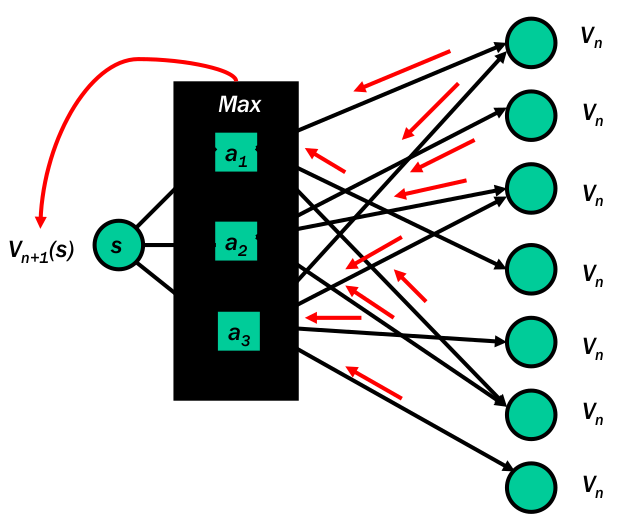
\includegraphics[width=0.3\linewidth]{images_pfe/Screenshot from 2024-06-14 17-08-41.png}
    \caption{Bellman Backup}
    \label{fig:Bellman-Backup}
\end{figure}
\section{Deep Reinforcement Learning}
\subsection{Reinforcement Learning}
Reinforcement Learning can be classified into two paradigms: model-based and model-free. In the case of model-based approaches, agents attempt to learn the transition function $T$, which can then be used when making action selections. By contrast, in the model-free approach, knowledge of T is not a requirement. Model-free learners instead sample
The underlying MDP is used to gain knowledge about the unknown model, in the form of
of value function estimates (Q values). These estimates represent the expected utility of each
state-action pair, which aids an agent in deciding which action is most desirable to select when in
a certain state.

An RL agent must find a balance between exploiting known good actions and exploring
the consequences of new actions to maximise the reward received during its lifetime. Two algorithms that are commonly used to manage the exploration-exploitation trade-off are
$\epsilon - \text{greedy}$ and softmax. The $\epsilon - \text{greedy}$ strategy selects the action with the highest expected value with probability $1 − \epsilon $, or a randomly selected action with the remaining probability $\epsilon $.


\subsection{Deep Q-Network}
\textbf{Q-learning} \parencite{Watkins} is one of the most commonly used RL algorithms. It is a model-free algorithm that has been shown to converge to the optimum action-values for an MDP with probability 1, so long as all actions in all states are sampled infinitely often and the
action-values are represented discretely. In practice, Q-learning will
learn good policies provided a sufficient number of samples are obtained for each state-action
pair. Agents implementing Q-learning update their Q values according to the following update rule:
\begin{equation}
    Q(s,a) \leftarrow Q(s,a) + \alpha [ r + \gamma max_{a'} Q(s',a') - Q(s,a)]
\end{equation}

Q values may be initialized in a number of different ways. The simplest method is to set the values for all state-action pairs to zero, i.e., \( \forall s, a \quad Q(s, a) = 0 \). Value function estimates may also be initialized using random values, \textbf{optimistic values}, or pessimistic values. \textbf{Optimistic initialization} sets the value for each state-action pair to the maximum possible reward; conversely, pessimistic initialization sets the value for each state-action pair to the minimum possible reward. The theoretical guarantees of Q-learning hold with any arbitrary initial Q values; therefore, the optimal policy for an MDP can be learned with any initial value function estimates.


Tabular representations are the simplest way to store value function estimates, where each state-action pair has a discrete \( Q \) value associated with it. When \( Q \) values are represented discretely, each additional feature tracked in the state leads to an exponential growth in the number of state-action pair values that must be stored \cite{Sutton1998}. This problem is commonly referred to in the literature as the \textbf{“curse of dimensionality”,} a term originally coined by Bellman \parencite{Bellman1957}. In simple environments, this is rarely an issue, but it may lead to an intractable problem in real-world applications due to memory or computational constraints. Learning over a large state-action space is possible, but it may take an unacceptably long time to learn useful policies. Alternatively, function approximation may be used to generalize across states and/or actions, whereby a \( Q \) function is used to store and retrieve estimates of the utility of state-action pairs. Function approximation, therefore, offers a way to mitigate against the state-action space explosion and is an active area of research in RL. Tile coding is one of the simplest forms of function approximation, where one tile represents multiple states or state-action pairs.


Neural Networks are also commonly used to implement Q functions, one of the most famous examples being Tesauro’s application of RL to backgammon (Tesauro 1994). It has been established that applied Deep Neural Networks can be a function approximation method; this emerging paradigm is known as \textbf{Deep Reinforcement Learning}. Deep RL has achieved human-level performance (or above) on complex tasks such as playing Atari games (Mnih et al. 2015) and playing the board game Go (Silver et al. 2016). Figure 2.1 shows a schematic of a DQN implemented in a Markov Decision Process. 

Tabular representations are used exclusively throughout this thesis for several reasons, including the fact that Q values must be represented discretely to preserve the theoretical guarantees offered by Q-learning \parencite{Watkins}. Although \textbf{reward shaping} could be applied in cases where function approximation is used, its use presents difficulties concerning developing theoretical guarantees for the techniques considered (Potential-based Reward Shaping and difference rewards).

\begin{figure}[hbt!]
  \centering
  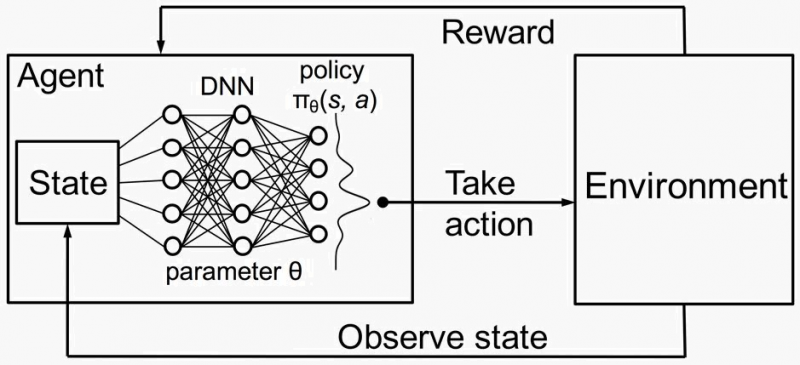
\includegraphics[width=0.5\textwidth]{images_pfe/1_ZZJ2FJFDNB9W-kdA2CfmTQ.png}
  \caption{DQN implementation in an MDP}
  \label{fig:dqn_mdp}
\end{figure}
\FloatBarrier

\textbf{Deep Q-Networks} (DQNs) build upon the principles of the Bellman Optimality equations, which are fundamental in RL. These equations describe how optimal value functions satisfy a recursive relationship, guiding the agent to maximize expected rewards over time. In practice, iterative methods like the Bellman backup are employed, where the equality in the Bellman Optimality equation is replaced with an update assignment:
\begin{equation}
    U_{i+1}(s) \leftarrow R(s) + \gamma \max_{a} \sum_{s'} T(s, a, s') U_i(s')
\end{equation}
This update, known as the \textbf{Bellman backup} (shown in \ref{fig: Bellman-Backup}), iteratively refines the estimate \( U_i(s) \) of the utility of state \( s \). The process continues until convergence, where \( U_i(s) \) approaches \( U^*(s) \), the optimal utility function, as \( i \) increases. DQNs leverage these principles to approximate the optimal action-value function \( Q^*(s, a) \) efficiently, using deep neural networks to approximate \( U_i(s) \) across large state spaces, thereby enabling complex decision-making in real-world applications of RL.

\subsection{From a Stochastic setting to a unique action}
An agent in a grid is always facing multiple choices when it comes to the actions it can take at any time step $t$, if we suppose the action space is $A=\{ 0,1,2,3,4 \} $, with: 
\begin{itemize}
    \item $0$: the agent stays in its previous state and does not move.
    \item $1$: the agent moves to the case that is adjacent to its right
    \item $2$: the agent moves to the case that is adjacent to its left
    \item $3$: the agent goes up
    \item $4$: the agent goes down
\end{itemize}
The current state of each agent is fed to the DQN as input. The information it holds gets encoded in the weights of the neurons of the DQN, and based on the current weights of the neural network, values are assigned to each of the actions $\{ 0,1,2,3,4 \} $. The final action that the agent chooses is through the \textbf{Maximum Expected Utility Principle:} The agent simply chooses the action that maximizes the expected utility of the subsequent state: 
\begin{equation}
    \pi (s) \in argmax _{a} \sum _{s'} T(s,a,s') U(s')
\end{equation}


\begin{figure}[hbt!]
  \centering
  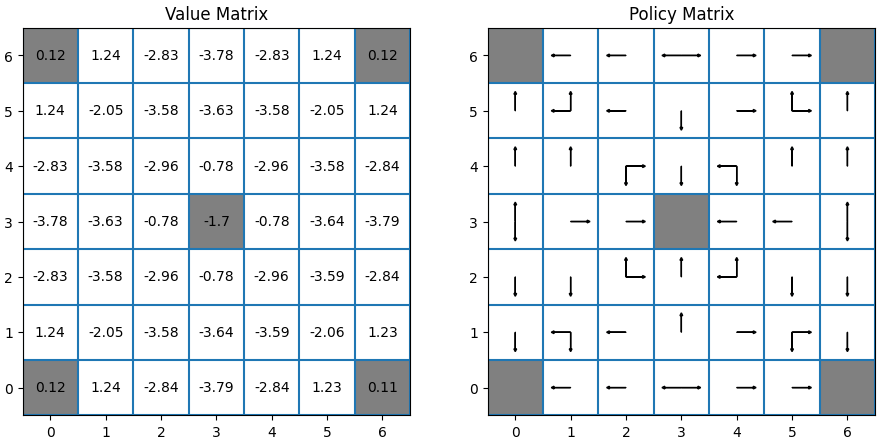
\includegraphics[width=0.7\textwidth]{images_pfe/1_tT9D_A8yJ0xkoul8e4H3Eg.png}
  \caption{Value Matrix and Policy Matrix for a Stochastic Setting (grid example).}
  \label{fig:value_policy_matrix_grid}
\end{figure}
\FloatBarrier

As shown in the figure above (\ref{fig:value_policy_matrix_grid}), the value of a state $s$ or the payoff of being in that state is represented by a number (eg.  $ 1.24, -0.78, \cdots $). The utility of a state is the immediate reward for that
state plus the expected discounted utility of the next
state, assuming that the agent chooses the optimal
action: 

\begin{equation}
    U(s) = R(s) + \gamma max _{a} \sum _{s'} T(s,a,s') U(s')
\end{equation}
This equation is the foundation of the \textbf{Bellman Backup principle}.

The state-action pairs values, or quality of taking an action $a_i$ given that the agent is in state $s$, is learned by the neural network using a \textbf{Loss function} that allows for the current DQN to converge to the Target DQN. Before the learning of the agents starts, both networks are initialized and are updated after each time step. The target network parameters $\theta^-$ are updated less frequently than the current network parameters $\theta$ to help stabilize training by providing consistent targets for a number of time steps. In literature, this is described as "DQN following its tail".


The loss function is mathematically expressed as:
\begin{equation}
    [
L(\theta) = \mathbb{E}_{(s, a, r, s') \sim \mathcal{D}} \left[ \left( y - Q(s, a; \theta) \right)^2 \right]
]
\end{equation}

Where:

\begin{itemize}
    \item $\theta$ are the parameters of the current Q-network.
    \item $\mathcal{D}$ is the replay buffer containing tuples $(s, a, r, s')$ of states, actions, rewards, and next states.
    \item $y$ is the target Q-value, defined as:
    \[
    y = r + \gamma \max_{a'} Q(s', a'; \theta^-)
    \]
    Here:
    \begin{itemize}
        \item $r$ is the reward received after taking action $a$ in state $s$.
        \item $\gamma$ is the discount factor.
        \item $\theta^-$ are the parameters of the target Q-network (which are periodically updated to match $\theta$).
    \end{itemize}
\end{itemize}

The \textbf{Replay Buffer ($\mathcal{D}$)} stores past experiences in the form of tuples $(s, a, r, s')$. During training, mini-batches of these experiences are sampled randomly to break the correlation between consecutive experiences, improving the stability and efficiency of learning. The \textbf{Target Q-Value ($y$)} is computed using the reward $r$ received plus the discounted maximum Q-value for the next state $s'$ using the target network. This incorporates the Bellman optimality equation to ensure that the network learns to predict future rewards accurately. And the \textbf{Loss Function} $L(\theta)$ is the mean squared error between the target Q-value $y$ and the predicted Q-value $Q(s, a; \theta)$ from the current Q-network. By minimizing this loss, the parameters $\theta$ of the current Q-network are adjusted to bring the predicted Q-values closer to the target Q-values.


\section{From Single-Agent to Multi-Agent Reinforcement Learning}
The principles of single-agent RL provide the building blocks for MARL. However, when multiple learning agents interact within a shared environment, the problem's complexity increases significantly. The environment's dynamics become dependent on the joint action of all agents, and each agent's success is tied to the behavior of others. This section formally introduces the models used in MARL and highlights the fundamental challenges that arise.

\subsection{The Formalism: Stochastic Games}
The standard single-agent MDP is insufficient to model a multi-agent system. The natural extension of the MDP to the multi-agent domain is the Stochastic Game (SG), also known as a Markov Game.

\begin{definition}[Stochastic Game]
A stochastic game is a tuple $\langle \mathcal{I}, S, \{A_i\}_{i \in \mathcal{I}}, T, \{R_i\}_{i \in \mathcal{I}}, \gamma \rangle$, where:
\begin{itemize}
    \item $\mathcal{I}$ is a finite set of $n$ agents, indexed by $i=1,...,n$.
    \item $S$ is the finite set of environment states.
    \item $A_i$ is the finite set of actions available to agent $i$. The joint action space is $A = A_1 \times \dots \times A_n$.
    \item $T: S \times A \times S \to [0,1]$ is the state transition probability function, which maps a state and a joint action to a distribution over next states.
    \item $R_i: S \times A \times S \to \mathbb{R}$ is the reward function for agent $i$.
    \item $\gamma \in [0,1]$ is the discount factor.
\end{itemize}
\end{definition}

At each timestep $t$, the system is in state $s_t \in S$. Each agent $i$ chooses an action $a_{i,t} \in A_i$, forming a joint action $a_t = (a_{1,t}, ..., a_{n,t}) \in A$. The environment then transitions to a new state $s_{t+1}$ with probability $T(s_{t+1} | s_t, a_t)$, and each agent $i$ receives a reward $r_{i,t}$.

The relationship between the agents' reward functions defines the nature of the game:

\paragraph{Fully Cooperative (Common-Reward)} All agents share the same reward function ($R_i = R_j$ for all $i,j$). Their goal is to collaborate to maximize this common reward. This is the setting for your project.

\paragraph{Fully Competitive (Zero-Sum)} The sum of rewards is always zero ($\sum_{i} R_i = 0$). One agent's gain is another's loss.

\paragraph{General-Sum} The most general case with no restrictions on the rewards. This can model mixed cooperative and competitive interactions.

\subsection{Core Challenges in MARL}
Moving from an MDP to an SG introduces fundamental challenges that render single-agent RL algorithms insufficient.

\subsubsection{Non-Stationarity}
% From the perspective of a single agent $i$, the environment is no longer stationary. The transition and reward dynamics depend on the actions of all other agents. As other agents update their policies $\pi_j$, the optimal policy for agent $i$ changes. This breaks the stationary Markov assumption
% that underpins algorithms like Q-learning, as the environment appears to be a constantly "moving target."
To any single agent, the environment seems unstable or non-stationary. This is because the result of its actions depends on the choices of all other agents. Since those other agents are also learning and constantly changing their strategies, the world becomes a \textbf{moving target}. An action that was good before might become bad now, breaking the stable environment assumption that is crucial for basic algorithms like Q-learning.
\subsubsection{Multi-Agent Credit Assignment}
 This challenge compounds the standard temporal credit assignment problem. In a cooperative setting, when a team receives a shared reward, it is highly non-trivial to determine the specific contribution of each individual agent's action to the team's success.
\subsubsection{Scalability}
 The joint action space of a multi-agent system often grows exponentially with the number of agents. This "curse of dimensionality" presents a significant barrier to scaling algorithms to systems with a very large number of agents.
\subsubsection{Partial Observability}
In most realistic scenarios, agents do not have access to the full environment state $s_t$. Instead, each agent $i$ receives a private, partial observation $o_{i,t}$ which contains incomplete information about $s_t$. This brings us to the most general framework for MARL, the Partially Observable Stochastic Game (POSG). For cooperative tasks, this is more specifically referred to as a Decentralized Partially Observable Markov Decision Process (Dec-POMDP).

\begin{definition}[Dec-POMDP]
A Dec-POMDP extends the Stochastic Game with observation components:
\begin{itemize}
    \item A set of observations for each agent, $\Omega_i$.
    \item An observation function $O: S \times A \to \mathcal{P}(\Omega)$ which gives the probability of a joint observation $o_t = (o_{1,t}, ..., o_{n,t})$ after a joint action $a_{t-1}$ leads to state $s_t$.
\end{itemize}
\end{definition}

Under partial observability, an agent cannot simply map its current observation to an optimal action. It must account for the history of its past observations to infer a belief about the true state of the environment. In deep RL, this is often achieved practically by equipping agent policies with memory, for example, by using Recurrent Neural Networks (RNNs) to process sequences of observations.\parencite{ma_deep_rl_challenges_and_applications}

Our project directly tackles this challenge of learning effective policies from partial observations in a cooperative setting.

% \subsubsection{The Goal: From Equilibrium to Coordination}
\subsubsection{From Equilibrium to Coordination}
In a general-sum SG, the solution is typically a Nash Equilibrium: a joint policy where no single agent can improve its own return by unilaterally changing its policy. However, in the fully cooperative (common-reward) setting of a Dec-POMDP, the objective is simpler and more direct: find the optimal joint policy $\pi^*$ that maximizes the shared expected return for the entire team.
$$ \pi^* = \arg\max_{\pi} \mathbb{E} \left[ \sum_{t=0}^{\infty} \gamma^t R(s_t, a_t, s_{t+1}) \right] $$
Solving this cooperative problem is the primary focus of the MARL algorithms we will discuss next, particularly those built on the CTDE paradigm.




% \subsection{Centralized Training with Decentralized Execution (CTDE)}
% Given the challenges of non-stationarity and partial observability, how can agents effectively learn to cooperate? A naive approach where each agent learns independently often fails because the environment is a \textbf{moving target.} The Centralized Training with Decentralized Execution (CTDE) paradigm offers an elegant and powerful solution.

% The core idea is to leverage different information structures during the training and execution phases:
% \begin{itemize}
%     \item \textbf{Centralized Training:} During the learning phase, the algorithm can access global information---such as the observations and actions of all agents---to train the policies more effectively. This privileged information helps overcome non-stationarity and aids credit assignment.
%     \item \textbf{Decentralized Execution:} After training, the centralized component is discarded. Each agent makes decisions using only its own local action-observation history, making the policies practical for real-world deployment.
% \end{itemize}

% \paragraph{The CTDE Actor-Critic Approach}
% A common way to implement CTDE is with an actor-critic architecture.

% \begin{description}
   

%     \item[The Actors (Decentralized Policies)] Each agent $i$ has its own policy, $\pi_i$, which is its actor. The actor is decentralized, mapping the agent's local action-observation history, $h_i$, to an action:
%     $$ \text{Actor}_i : \pi_i(a_i | h_i) $$
    
%     \item[The Critic (Centralized Value Function)] A single, centralized critic is used during training to evaluate the joint actions of the team. This critic is an action-value function, $Q_{\pi}(h,a)$, that takes the joint history $h = \langle h_1, \dots, h_n \rangle$ and joint action $a$ as input.
% \end{description}
% Formally, for a given joint policy $\pi$, this centralized Q-function represents the total expected discounted reward from taking joint action $a$ in joint history $h$ and following the joint policy $\pi$ thereafter. It can be defined recursively:
% $$ Q_{\pi}(h,a) = \sum_{s \in S} P(s|h) \left( R(s,a) + \gamma \sum_{s' \in S} T(s'|s,a) \sum_{o \in \Omega} O(o|s',a) V_{\pi}(hao) \right) $$
% where $V_{\pi}(hao)$ is the value of the next joint history.

% In practice, an RL algorithm does not compute this expectation exactly. Instead, it approximates the critic's value through sampling from experiences collected during training. The goal of the centralized critic is to provide a stable and high-quality learning signal to the actors.

% During training, the agents follow their local actors to generate experience. The centralized critic evaluates this experience and guides the updates for each decentralized actor, effectively telling the team which joint behaviors lead to success. After training, the complex critic is discarded, leaving only the efficient decentralized actors for execution. This framework is the foundation for many state-of-the-art cooperative MARL algorithms.
\subsection{Centralized Training with Decentralized Execution (CTDE)}
Given the challenges of non-stationarity and partial observability, a naive approach where each agent learns independently often fails because the environment is a constantly moving target. The CTDE paradigm offers an elegant and powerful solution.

The core idea is to leverage different information structures during the training and execution phases:
\begin{itemize}
    \item \textbf{Centralized Training:} During the learning phase, the algorithm can access privileged, global information, such as the observations and actions of all agents. This stable, global view is used to train the agent policies more effectively, which overcomes the non-stationarity problem and aids in the credit assignment challenge.
    \item \textbf{Decentralized Execution:} After training, the centralized component is discarded. Each agent makes decisions using only its own local action-observation history. This ensures the resulting policies are practical, lightweight, and can be deployed in the real world where global information is unavailable.
\end{itemize}
\subsection{CTDE Implementation Paradigms}
The CTDE framework is primarily realized through two dominant strategies, which are defined by how the centralized training is performed.

\subsubsection{Value-Based CTDE}
In value-based CTDE algorithms, the dominant strategy is value decomposition. This approach focuses on learning the global action-value function, $Q_{\text{tot}}$, by factorizing it into a set of individual utility functions, $Q_i$, one for each agent. The core principle is that the centralized $Q_{\text{tot}}$ is learned as a non-linear combination of the per-agent values, which are learned using only local observations. The main design challenge is to structure this combination to ensure that selecting the best local action for each agent also yields the best joint action for the team. This allows for optimal decentralized execution while learning a complex, centralized team-value function. This paradigm is the foundation for popular cooperative algorithms like VDN\parencite{VDN} and QMIX\parencite{QMIX}.

\subsubsection{Policy-Gradient-Based CTDE}
Another major branch of CTDE involves policy-gradient methods. This paradigm applies the actor-critic model more directly. Each agent learns its own policy, $\pi_i$ (the actor), while a centralized critic learns a value function, $Q(s,a)$, to evaluate the team's performance. During training, the critic leverages global information (the full state $s$ and the joint action $a$) to compute an accurate and low-variance policy gradient for each individual actor. This gradient signal then guides the updates for each agent's policy, effectively teaching each actor how its actions contribute to the team's success. The canonical example of this approach is the Multi-Agent Deep Deterministic Policy Gradient (MADDPG) algorithm\parencite{MADDPG}.
The most common implementation of this paradigm is through an actor-critic framework:
\begin{description}
    \item[The Actors (Decentralized Policies)] Each agent $i$ has its own policy, $\pi_i$, which is its actor. The actor is decentralized, mapping the agent's local action-observation history, $h_i$, to an action: $\pi_i(a_i|h_i)$.
    \item[The Critic (Centralized Value Function)] A single, centralized critic, typically an action-value function $Q_{\text{tot}}(h,a)$, is used during training to evaluate the joint actions of the team based on global information.
\end{description}
% During training, the powerful centralized critic guides the updates for all the simple, decentralized actors. After training is complete, the complex critic is discarded, leaving only the efficient decentralized actors for execution.
The CTDE paradigm is commonly implemented using an actor-critic \parencite{ppo_ctde} architecture, which can be conceptually understood through an analogy to teacher-student learning models. In this framework, the centralized critic acts as the \textit{teacher}\parencite{CTDS}. It is a network utilized only during the training phase, with access to global information such as the true state of the environment ($s$) or the joint action-observation history. This global perspective allows it to compute a stable, low-variance learning signal.

The decentralized actors are analogous to the \textit{students}; they are the individual policies ($\pi_i$) for each agent, designed to operate solely on local observations ($o_i$). During training, the critic evaluates the joint actions taken by the actors and computes a precise learning signal [Temporal Difference (TD) error]. This signal is then used to guide the policy updates for each decentralized actor, effectively teaching the agents how to coordinate.
\begin{figure}[hbt!]
    \centering
     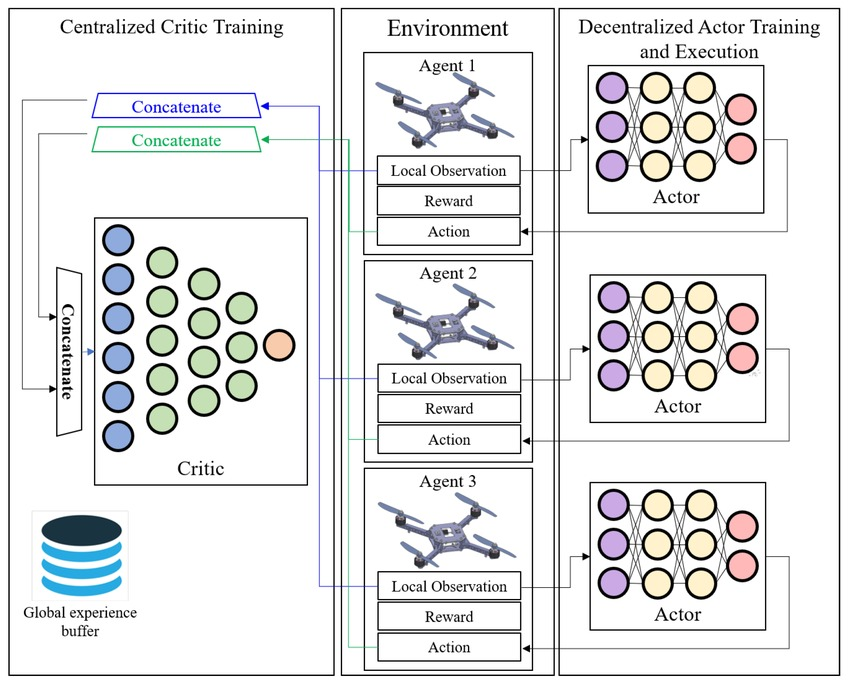
\includegraphics[width=0.4\textwidth]{img_pfe/ctde.jpeg}
    \caption{CTDE MARL framework for collaborative UAV swarm navigation.
   \parencite{swarm_navigation_ctde} }.
    \label{fig:ctde}
\end{figure}

Once training converges, the computationally expensive centralized critic is discarded. The final product is a set of efficient, decentralized actors capable of effective performance during execution, making the approach both powerful in training and practical in deployment.

\subsection{Key Assumptions of the CTDE Paradigm}
The popular CTDE paradigm, while powerful, relies on its own set of strong assumptions to function effectively.
\begin{itemize}
  \item Centralized Access During Training: The primary assumption is that a centralized controller can access global information (e.g., the full state or all agents' observations and actions) during a simulated training phase. This allows for efficient, coordinated learning, but may not be feasible in real-world scenarios where such a centralized simulator is unavailable.
    \item Factorizability of the Joint Value Function: Value-based CTDE methods, such as VDN and QMIX, assume that the team's joint action-value function ($Q_{\text{tot}}$) can be effectively represented as a combination of individual agent utilities ($Q_i$). This factorization is crucial for decentralized execution, but if the problem's true value function cannot be represented this way, these methods may fail to converge to the optimal policy.
\end{itemize}

\begin{figure}[H]
    \centering
   
        
    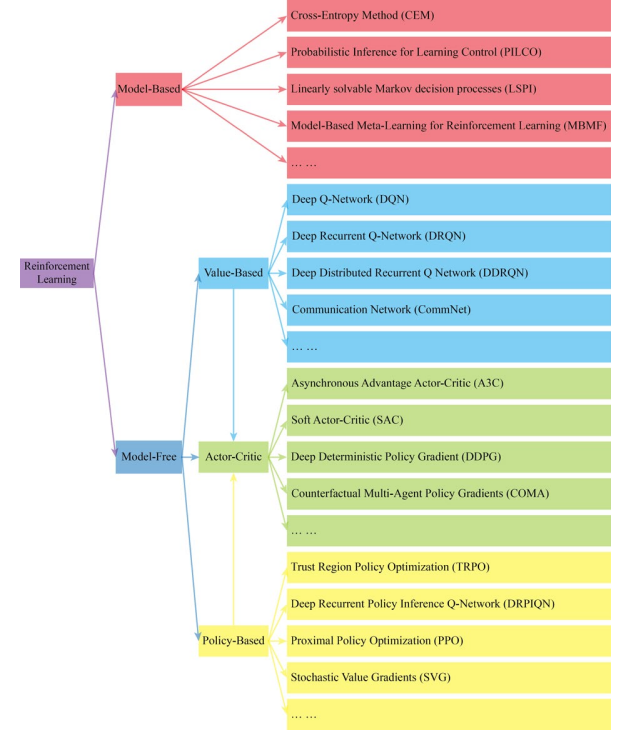
\includegraphics[width= 0.6\linewidth]{img_pfe/Classification_of_RL.PNG}
                \caption{Classification of reinforcement learning algorithms (Adapted from \parencite{smacv2_review})}
        \label{fig:classification_of_RL}
\end{figure}
    
\section*{Conclusion}

This chapter has charted a course from the well-defined world of single-agent reinforcement learning to the complex, dynamic frontier of multi-agent systems. We began with foundational principles, then journeyed into the multi-agent domain, where interacting learners give rise to profound challenges like non-stationarity and partial observability. In response, powerful frameworks like CTDE have emerged. However, we have also seen that CTDE is not a complete solution, as it introduces its own theoretical gaps related to scalability, representation, and factorization. It is precisely these gaps, especially the challenge of forming effective policies from limited, partial observations, that provide the motivation for our work in this report. Having established this theoretical landscape, we are now equipped to explore the state-of-the-art algorithms that attempt to navigate these complexities, before introducing our own proposed solution.